\begin{ReasoningBox}[title=Qualitative Decision Making] % 可以通过 title 参数修改标题
    % --- 第一部分：问题描述与图片 ---
    % \begin{minipage}[t]{0.58\textwidth}
    \begin{wrapfigure}{r}{0.5\textwidth}
        \centering
        % wrapfigure 通常顶部会有多余空白，使用负 vspace 向上提，让图片和第一行文字对齐
        \vspace{-20pt} 
        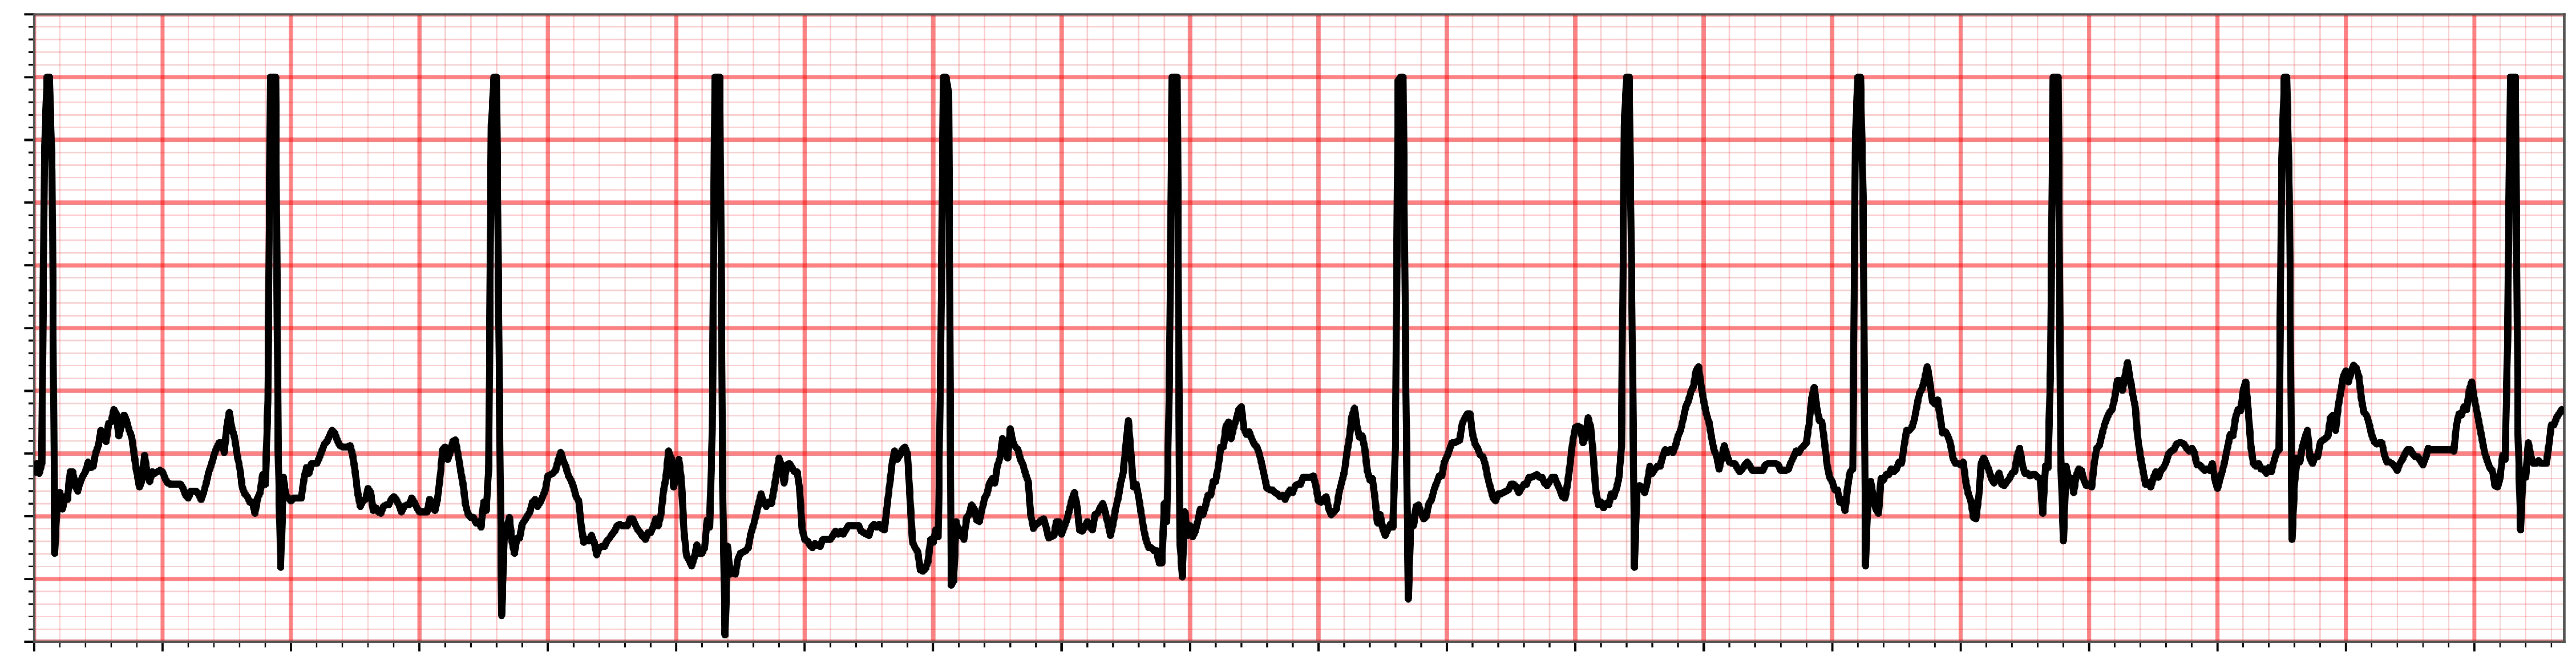
\includegraphics[width=\linewidth]{blocks/sample_cases_success/ECG.pdf}
        % 调整底部的留白
        \vspace{-20pt}
    \end{wrapfigure}
\textbf{Question:} You are an expert cardiologist specializing in ECG interpretation and diagnosis of cardiovascular diseases. Your task is to analyze the 12-lead ECG signals and make clinical treatment decisions based on:\\1. **Signal Pattern Recognition**: Identify pathological waveforms (ST elevation/depression, T-wave inversions, Q waves, QRS morphology) across all leads to recognize acute ischemia, infarction, or conduction abnormalities.\\2. **Anatomical Correlation**: Recognize which leads correspond to specific cardiac regions (inferior, anterior, lateral, septal walls) to localize the affected myocardial territory and implicated coronary artery.\\3. **Clinical Reasoning**: Integrate ECG findings with your knowledge of cardiac pathophysiology to determine disease acuity (emergent vs urgent vs elective) and appropriate treatment pathway (urgent reperfusion, ACS protocol, monitoring, medication adjustment).\\4. **Differential Diagnosis**: Consider multiple conditions that could produce similar ECG patterns and select the most appropriate treatment based on the overall clinical picture and established guidelines (AHA/ACC/ESC).\\The time-series data represents normalized ECG signals sampled at 100 Hz. Each of the 12 leads provides a different electrical view of the heart's activity. Analyze the morphology, amplitude, duration, and spatial distribution of waveforms systematically to guide evidence-based clinical decisions.\\
Based on the 12-lead ECG analysis above and the provided signal data, what is the most appropriate clinical management?
    \vspace{0.5em}

    % --- 第二部分：选项 ---
    \textbf{Answer Choices:} \\ 
    (A) Clinical correlation; repeat ECG and consider stress test \\
    (B) Assess for hypertension; initiate antihypertensive therapy; echo \\
    (C) Monitor; often a benign variant, but assess if symptomatic \\
    (D) Monitor digoxin levels; assess for toxicity (arrhythmias, GI, visual) \\
    \textbf{Correct Answer:} \textcolor{correctgreen}{(A)} \\
\end{ReasoningBox}